\chapter{Data Collection}
\label{sec:Data_Collection}

The data collection portion of this project is immediately tasked with the following set of problems: spatial coincidence, temporal coincidence, and resolution. Given the asynchronous orbits of each satellite and the incompatible resolutions of ESA's SN-2 and NASA's IS-2, other avenues were explored to obtain precise SAR imaging. Of note were NASA's "ICESAT-2" mobile application and ICEYE's\textsuperscript{\tiny\textcopyright} SAR imaging offered through the ESA.

\section {SAR Imaging}
The resolution incompatibility between SAR and LiDAR instruments could not be resolved by the data made freely available by the ESA or NASA. However, the ESA offers to sponsor data from third party companies through their Earth Observation User Services Portal. Companies like ICEYE, which offer SAR data products at up to .01m resolution, provide SAR imagery that is significantly more compatible with IS-2's small footprint in comparison to the free alternatives.

To achieve ESA sponsorship of this data, a proposal was submitted including the objective of the project, researchers involved in the task, which satellite and product was being requested, and a general plan outlining the use of the sponsored data. Given the latency of proposal approval, and the seasonal characteristics of arctic sea ice, alternate efforts to coincide freely available SN-2 10m resolution data with IS-2's altimetry.

Referring to ESA's Copernicus Open Access Hub and NASA's Earthdata Search tool, a near coincident set of SN-2 and IS-2 data was obtained for February 20-21 of 2023 (Figure 2.1). The SAR imaging clearly captured regions of arctic ice, and did so on February 20th at 4:50pm local time. The predominantly spatially coincident IS-2 measurements, being the long purple and orange tracks in the figure, crossed the region at 10am and 10pm local time on February 21. This data while immensely geographically coincident, was doubtful given its 17 and 29 hour respective temporal delay. Utility scripts were devised to track buoy movement in the area across the time period, and the nearest buoy (purple) to any of the tracks was 30 kilometers away and had traveled another 8 km during the data's time difference. The corroboration of buoy data invalidates the possibility of validity of the data, as it's unreasonable to account for the drift of the ice over the given time and space scale. While unsuccessful, this instance demonstrates the inavailability of naturally coincident data and the ineffeciencies involved in obtaining it.

\begin{figure}
    \centering
	\includegraphics[width=.8\textwidth]{../research-resources/ice-sat-2/near-coincidence-buoys.png}
    \label{near-coincidence}%
\end{figure}



\begin{figure}
    \centering
    \subfigure[]{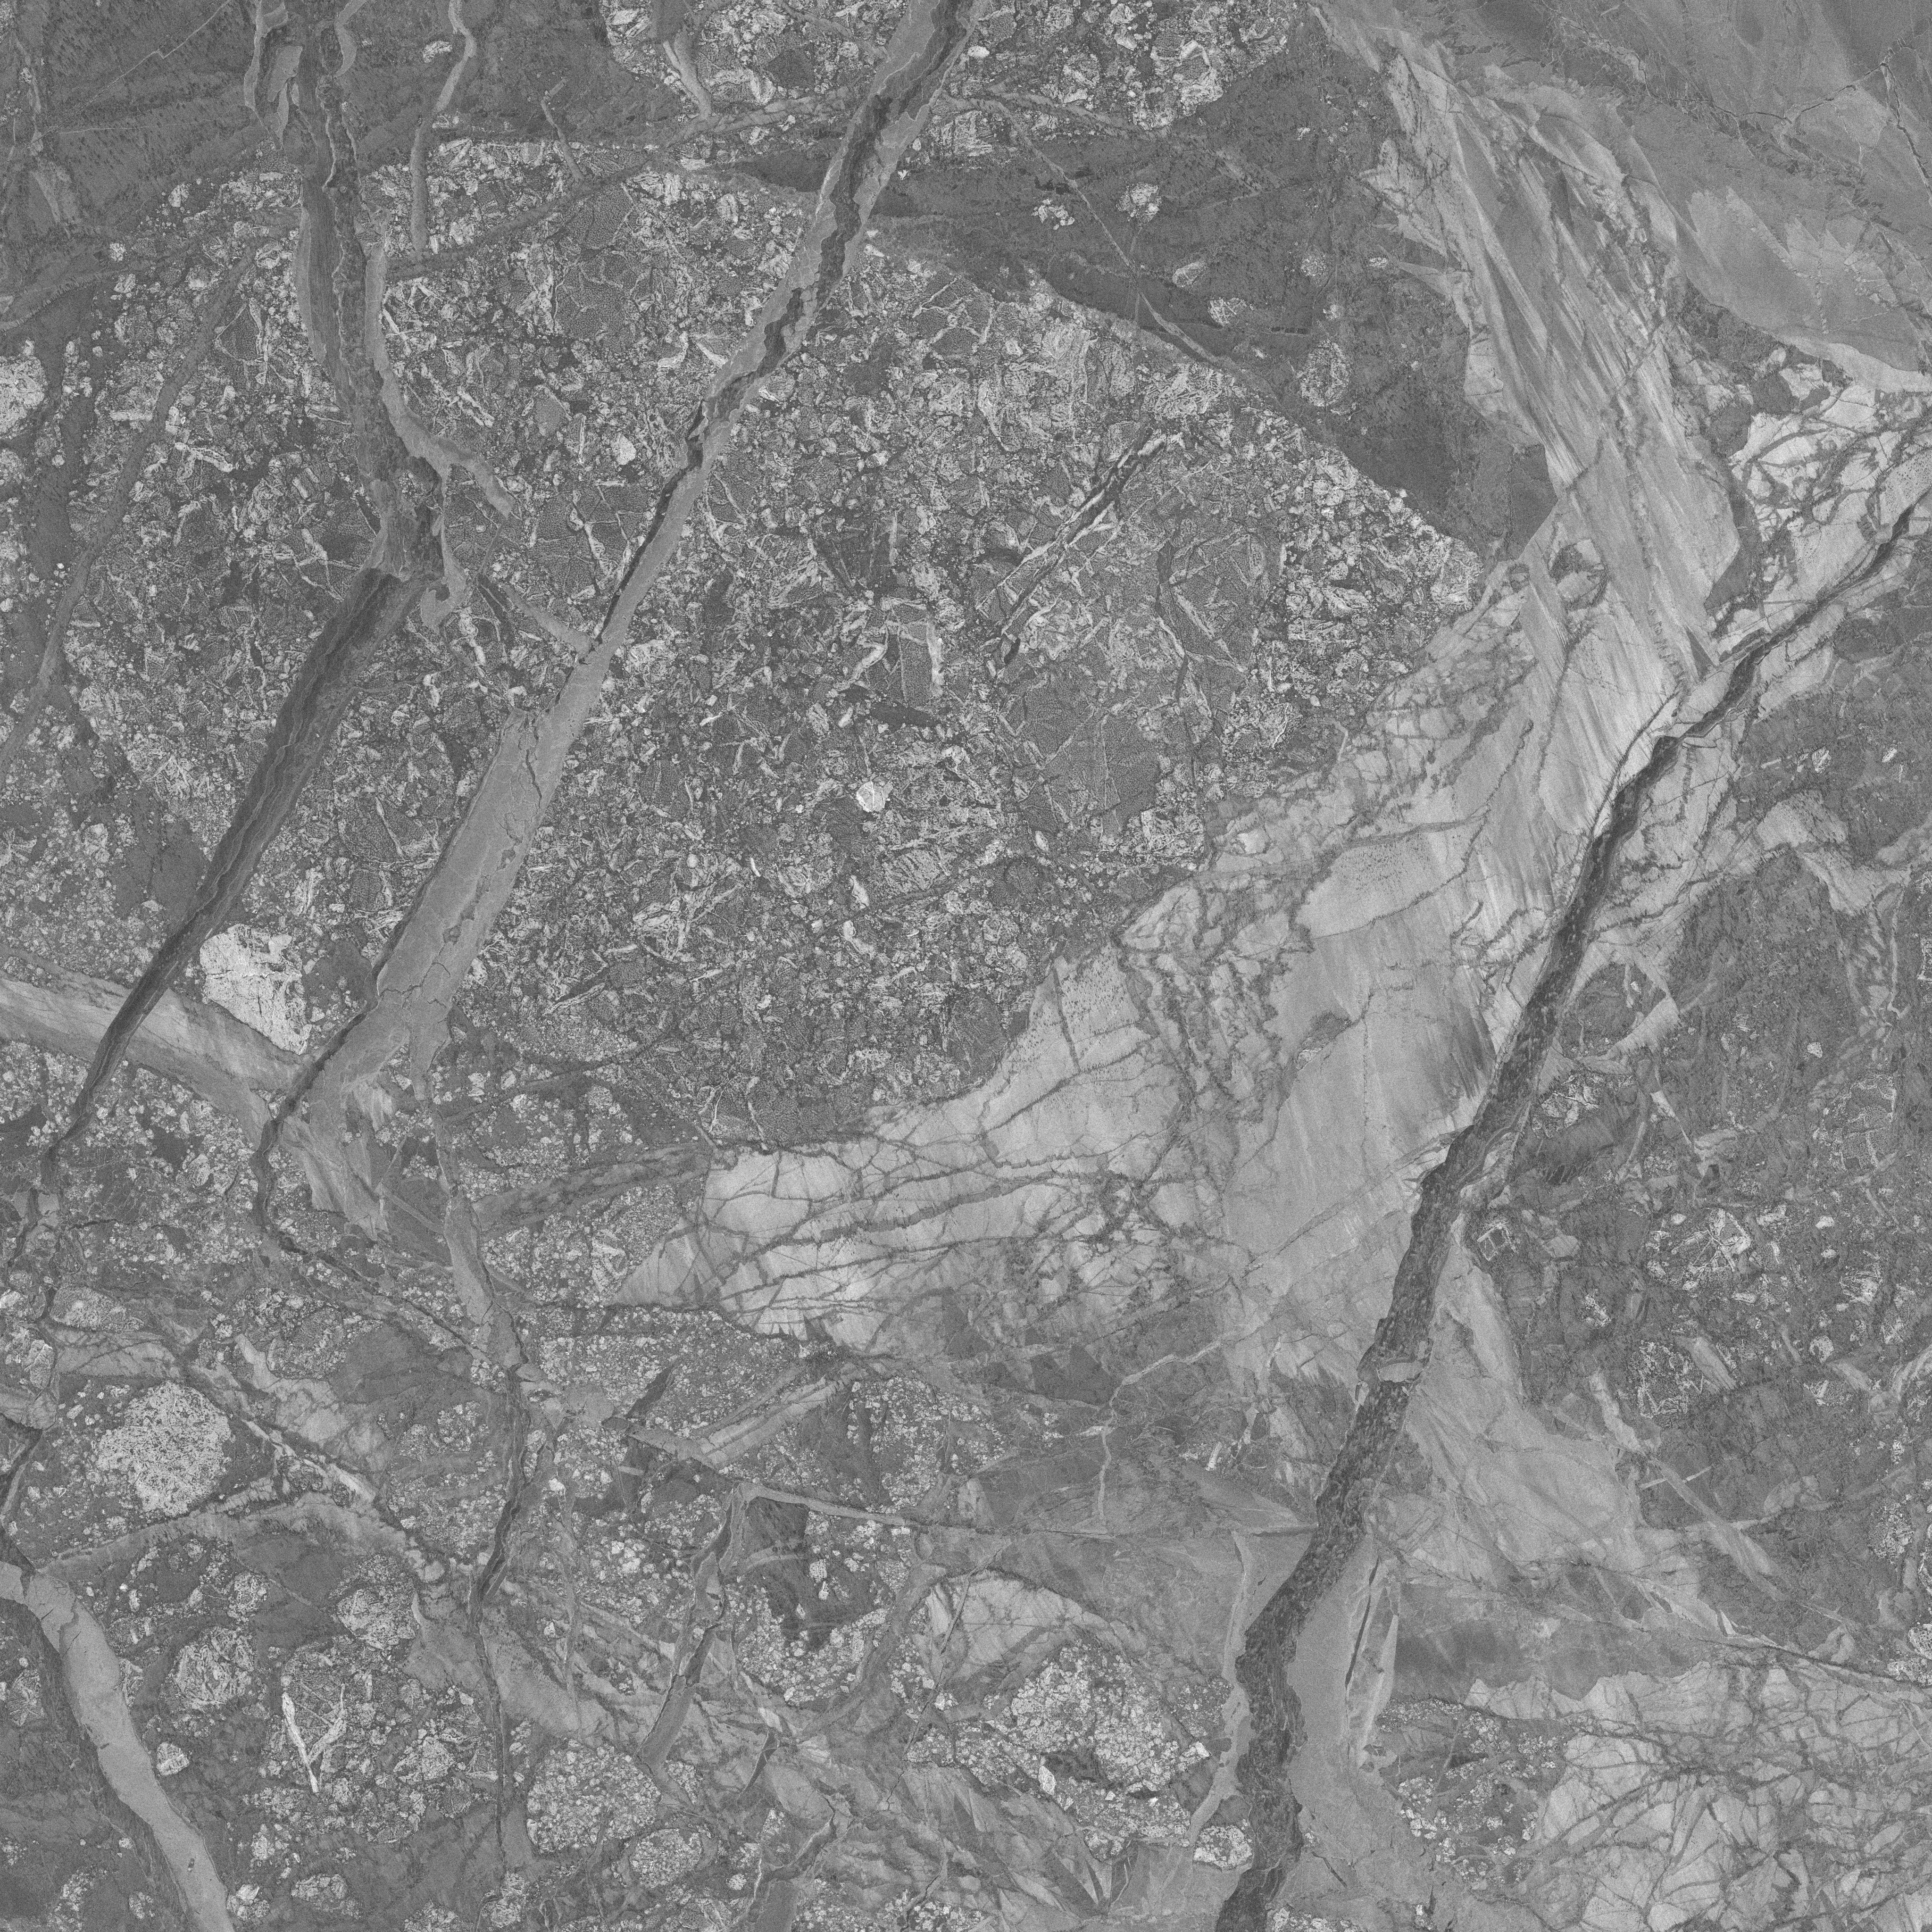
\includegraphics[width=.48\linewidth]{./research-resources/SAR/ICEYE_X2_QUICKLOOK_SLEA_3279211_20240119T044029.png}}
    \subfigure[]{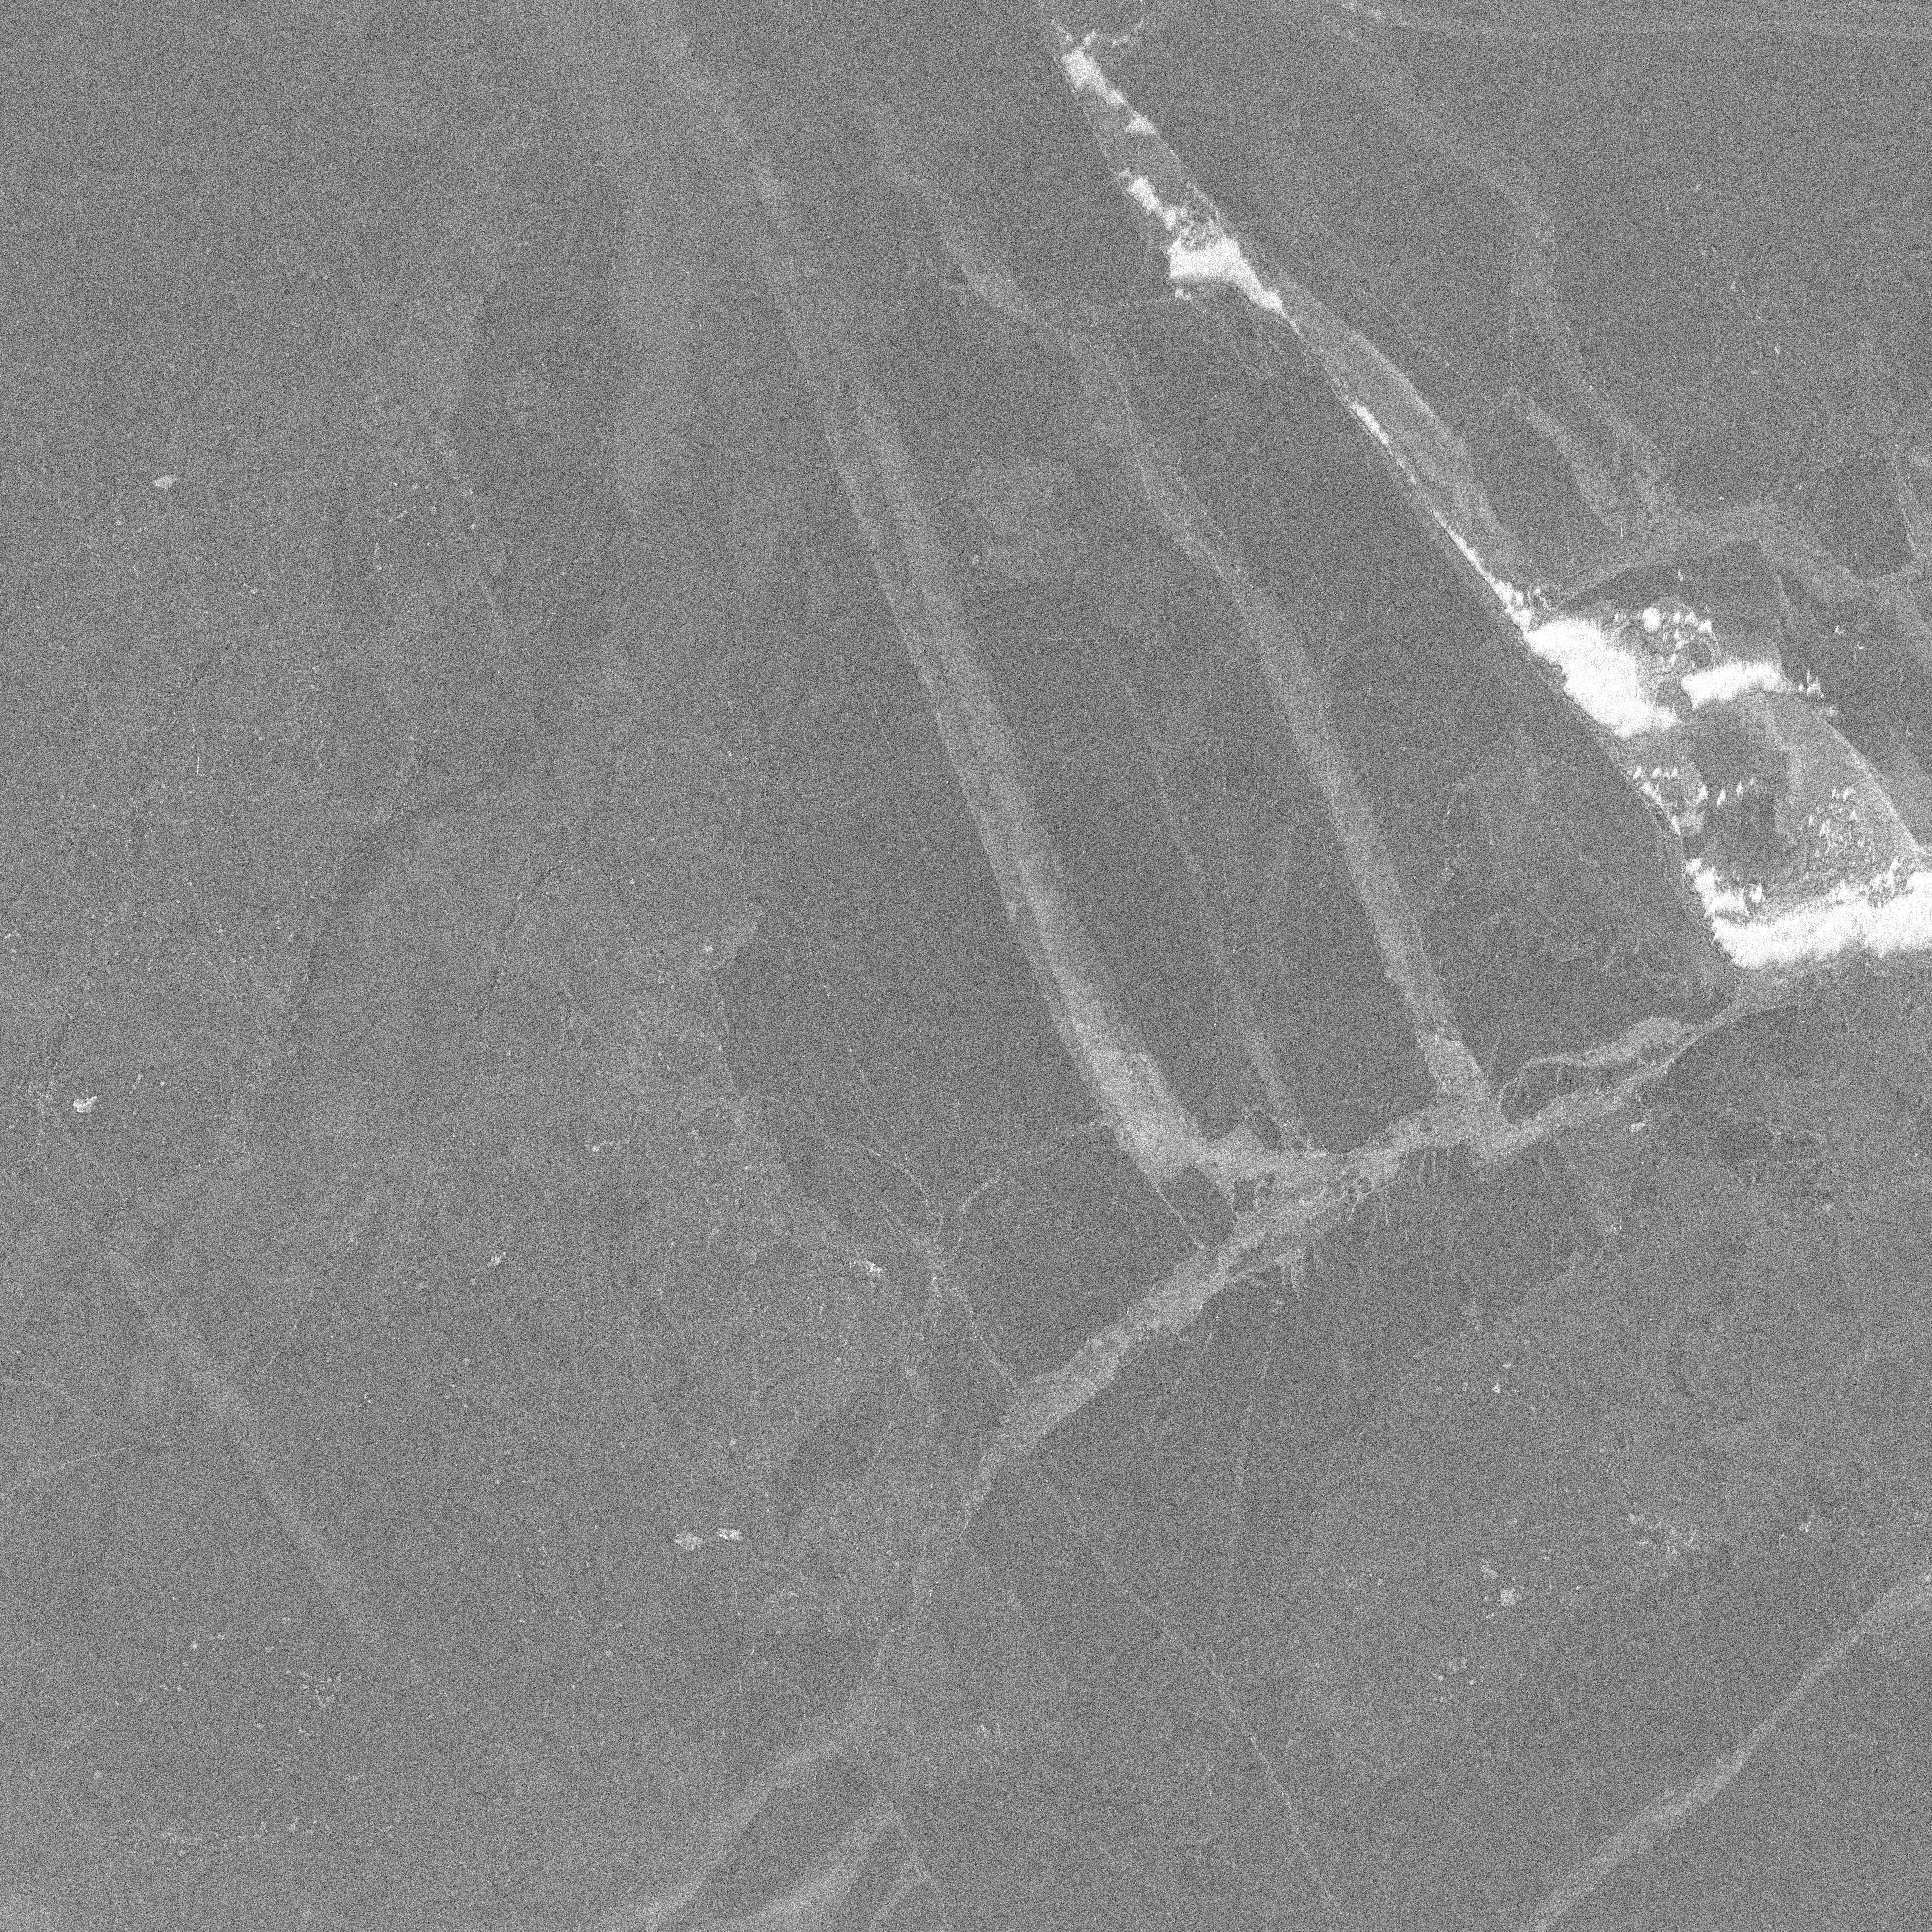
\includegraphics[width=.48\linewidth]{./research-resources/SAR/ICEYE_X6_QUICKLOOK_SLH_3280232_20240120T132858.png}}
    \subfigure[]{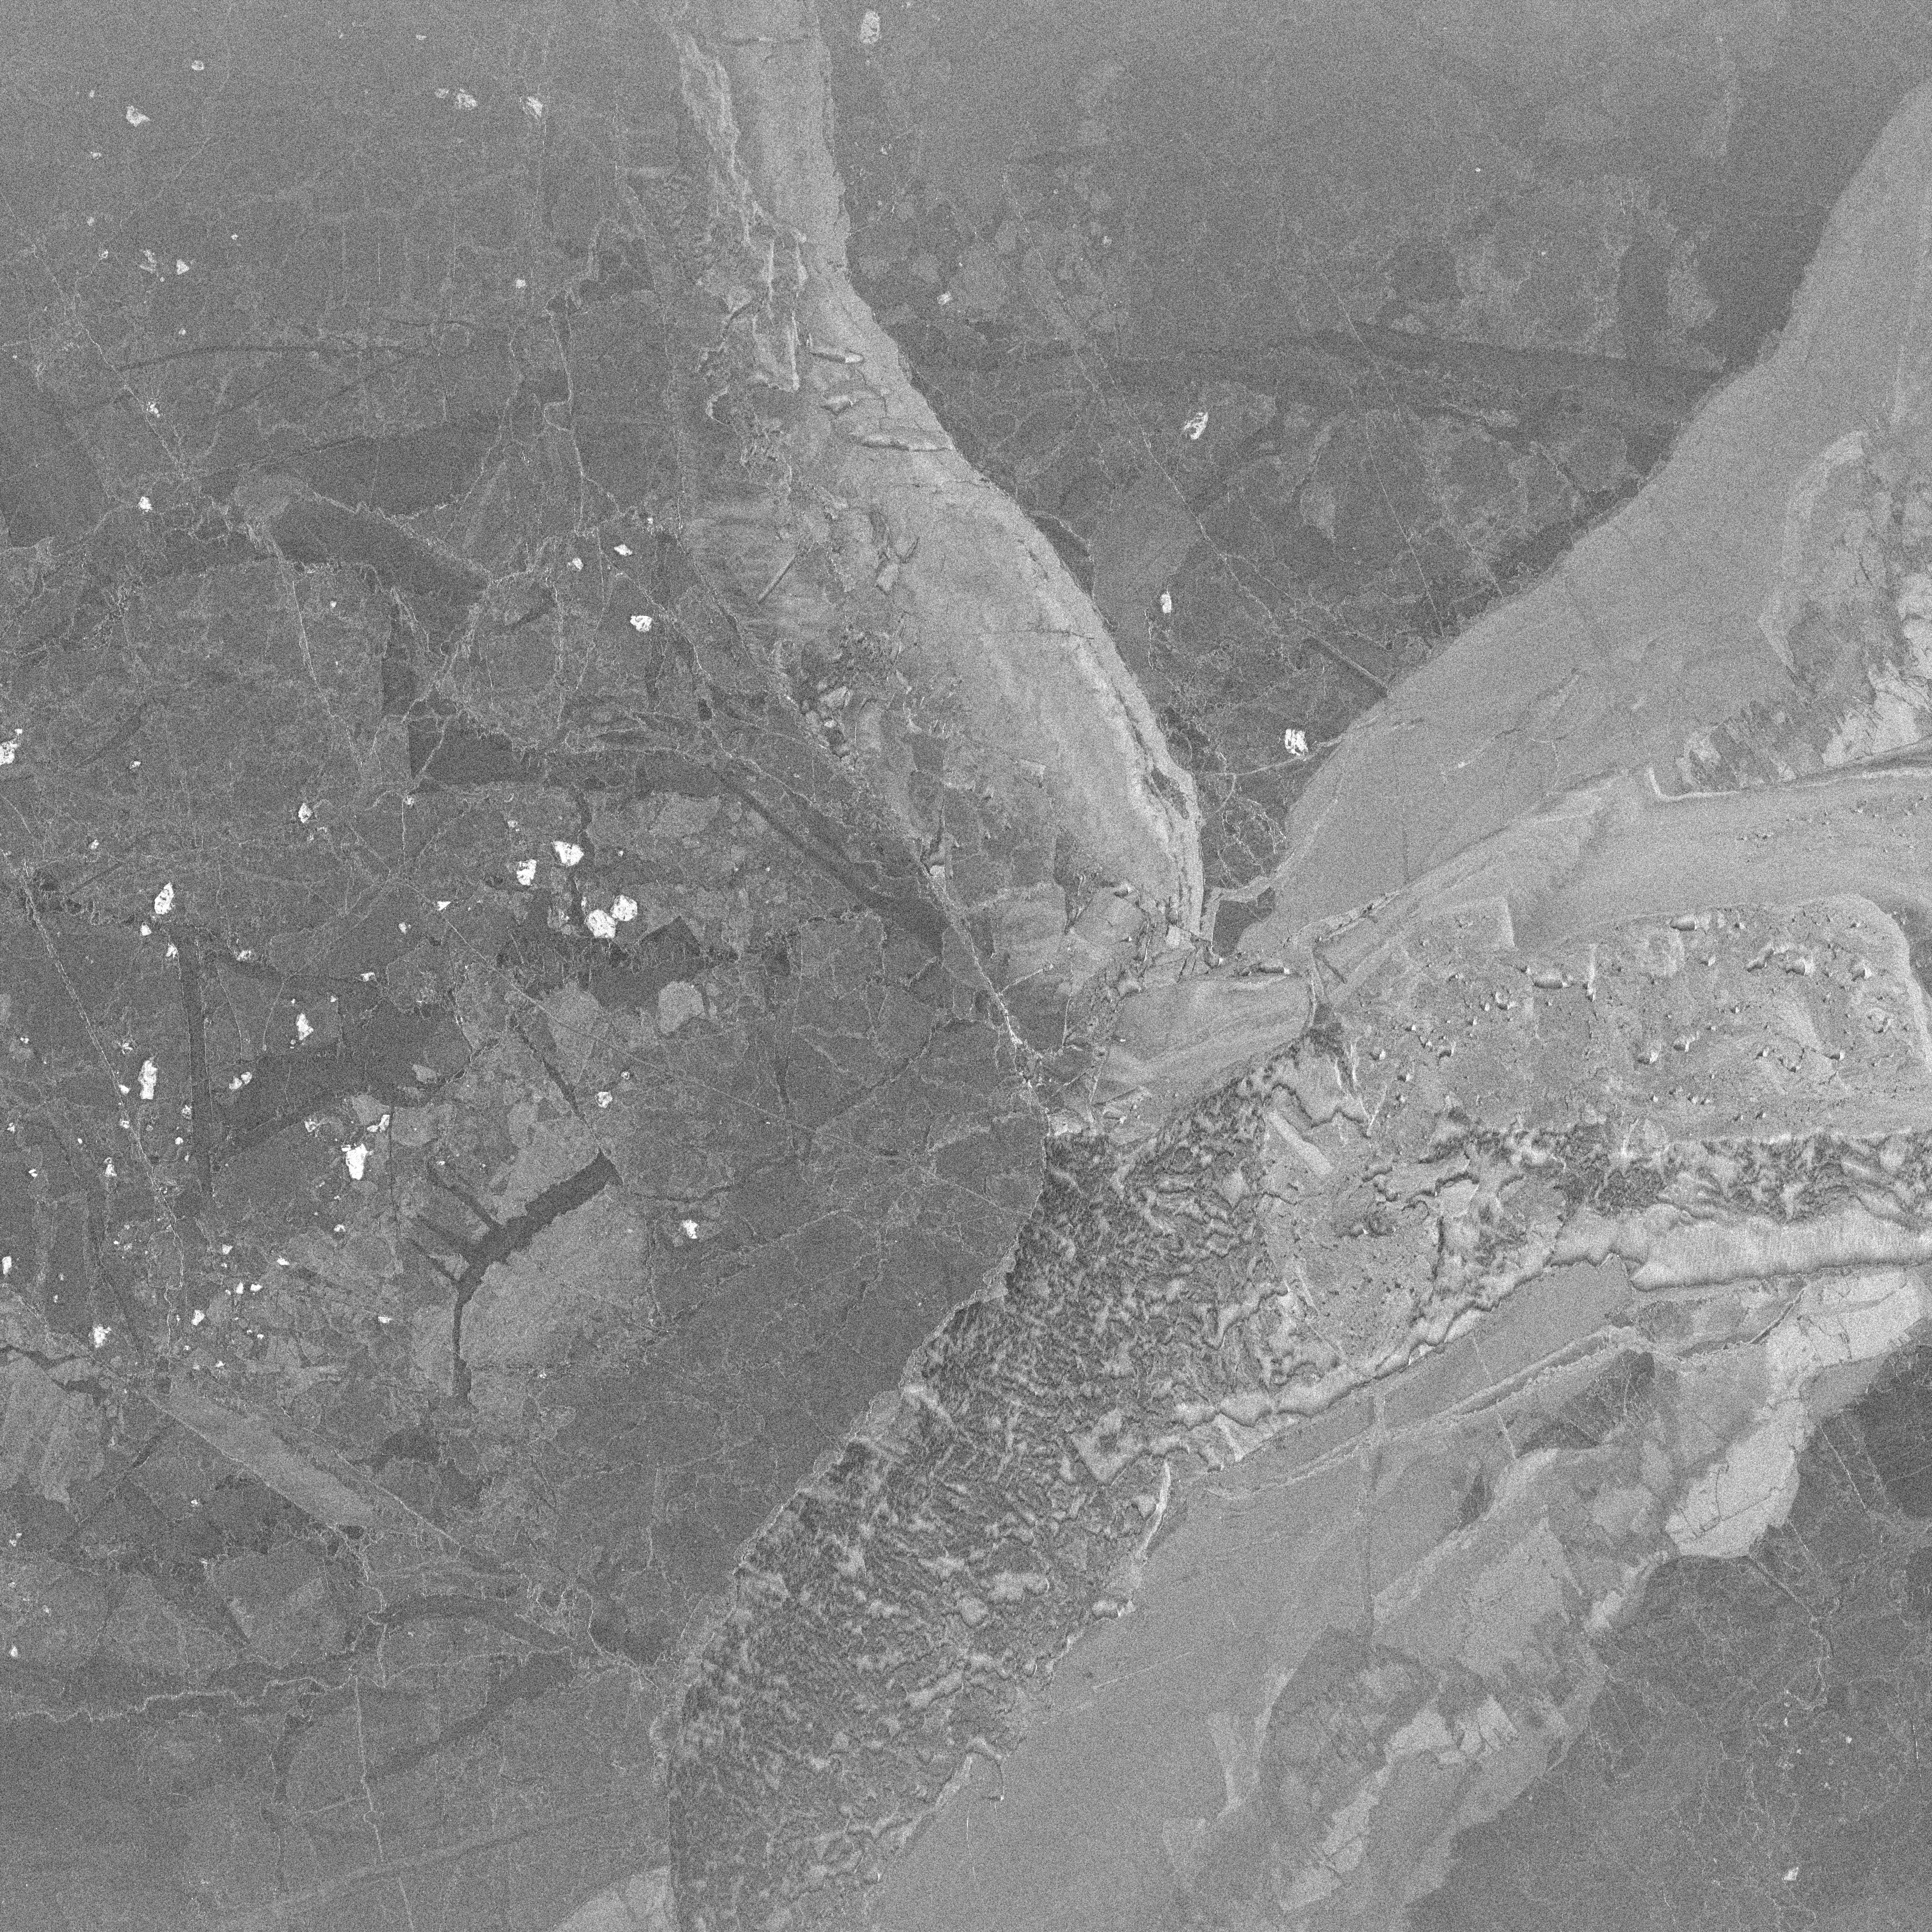
\includegraphics[width=.48\linewidth]{./research-resources/SAR/ICEYE_X8_QUICKLOOK_SLH_3295462_20240120T202547.png}}
    \subfigure[]{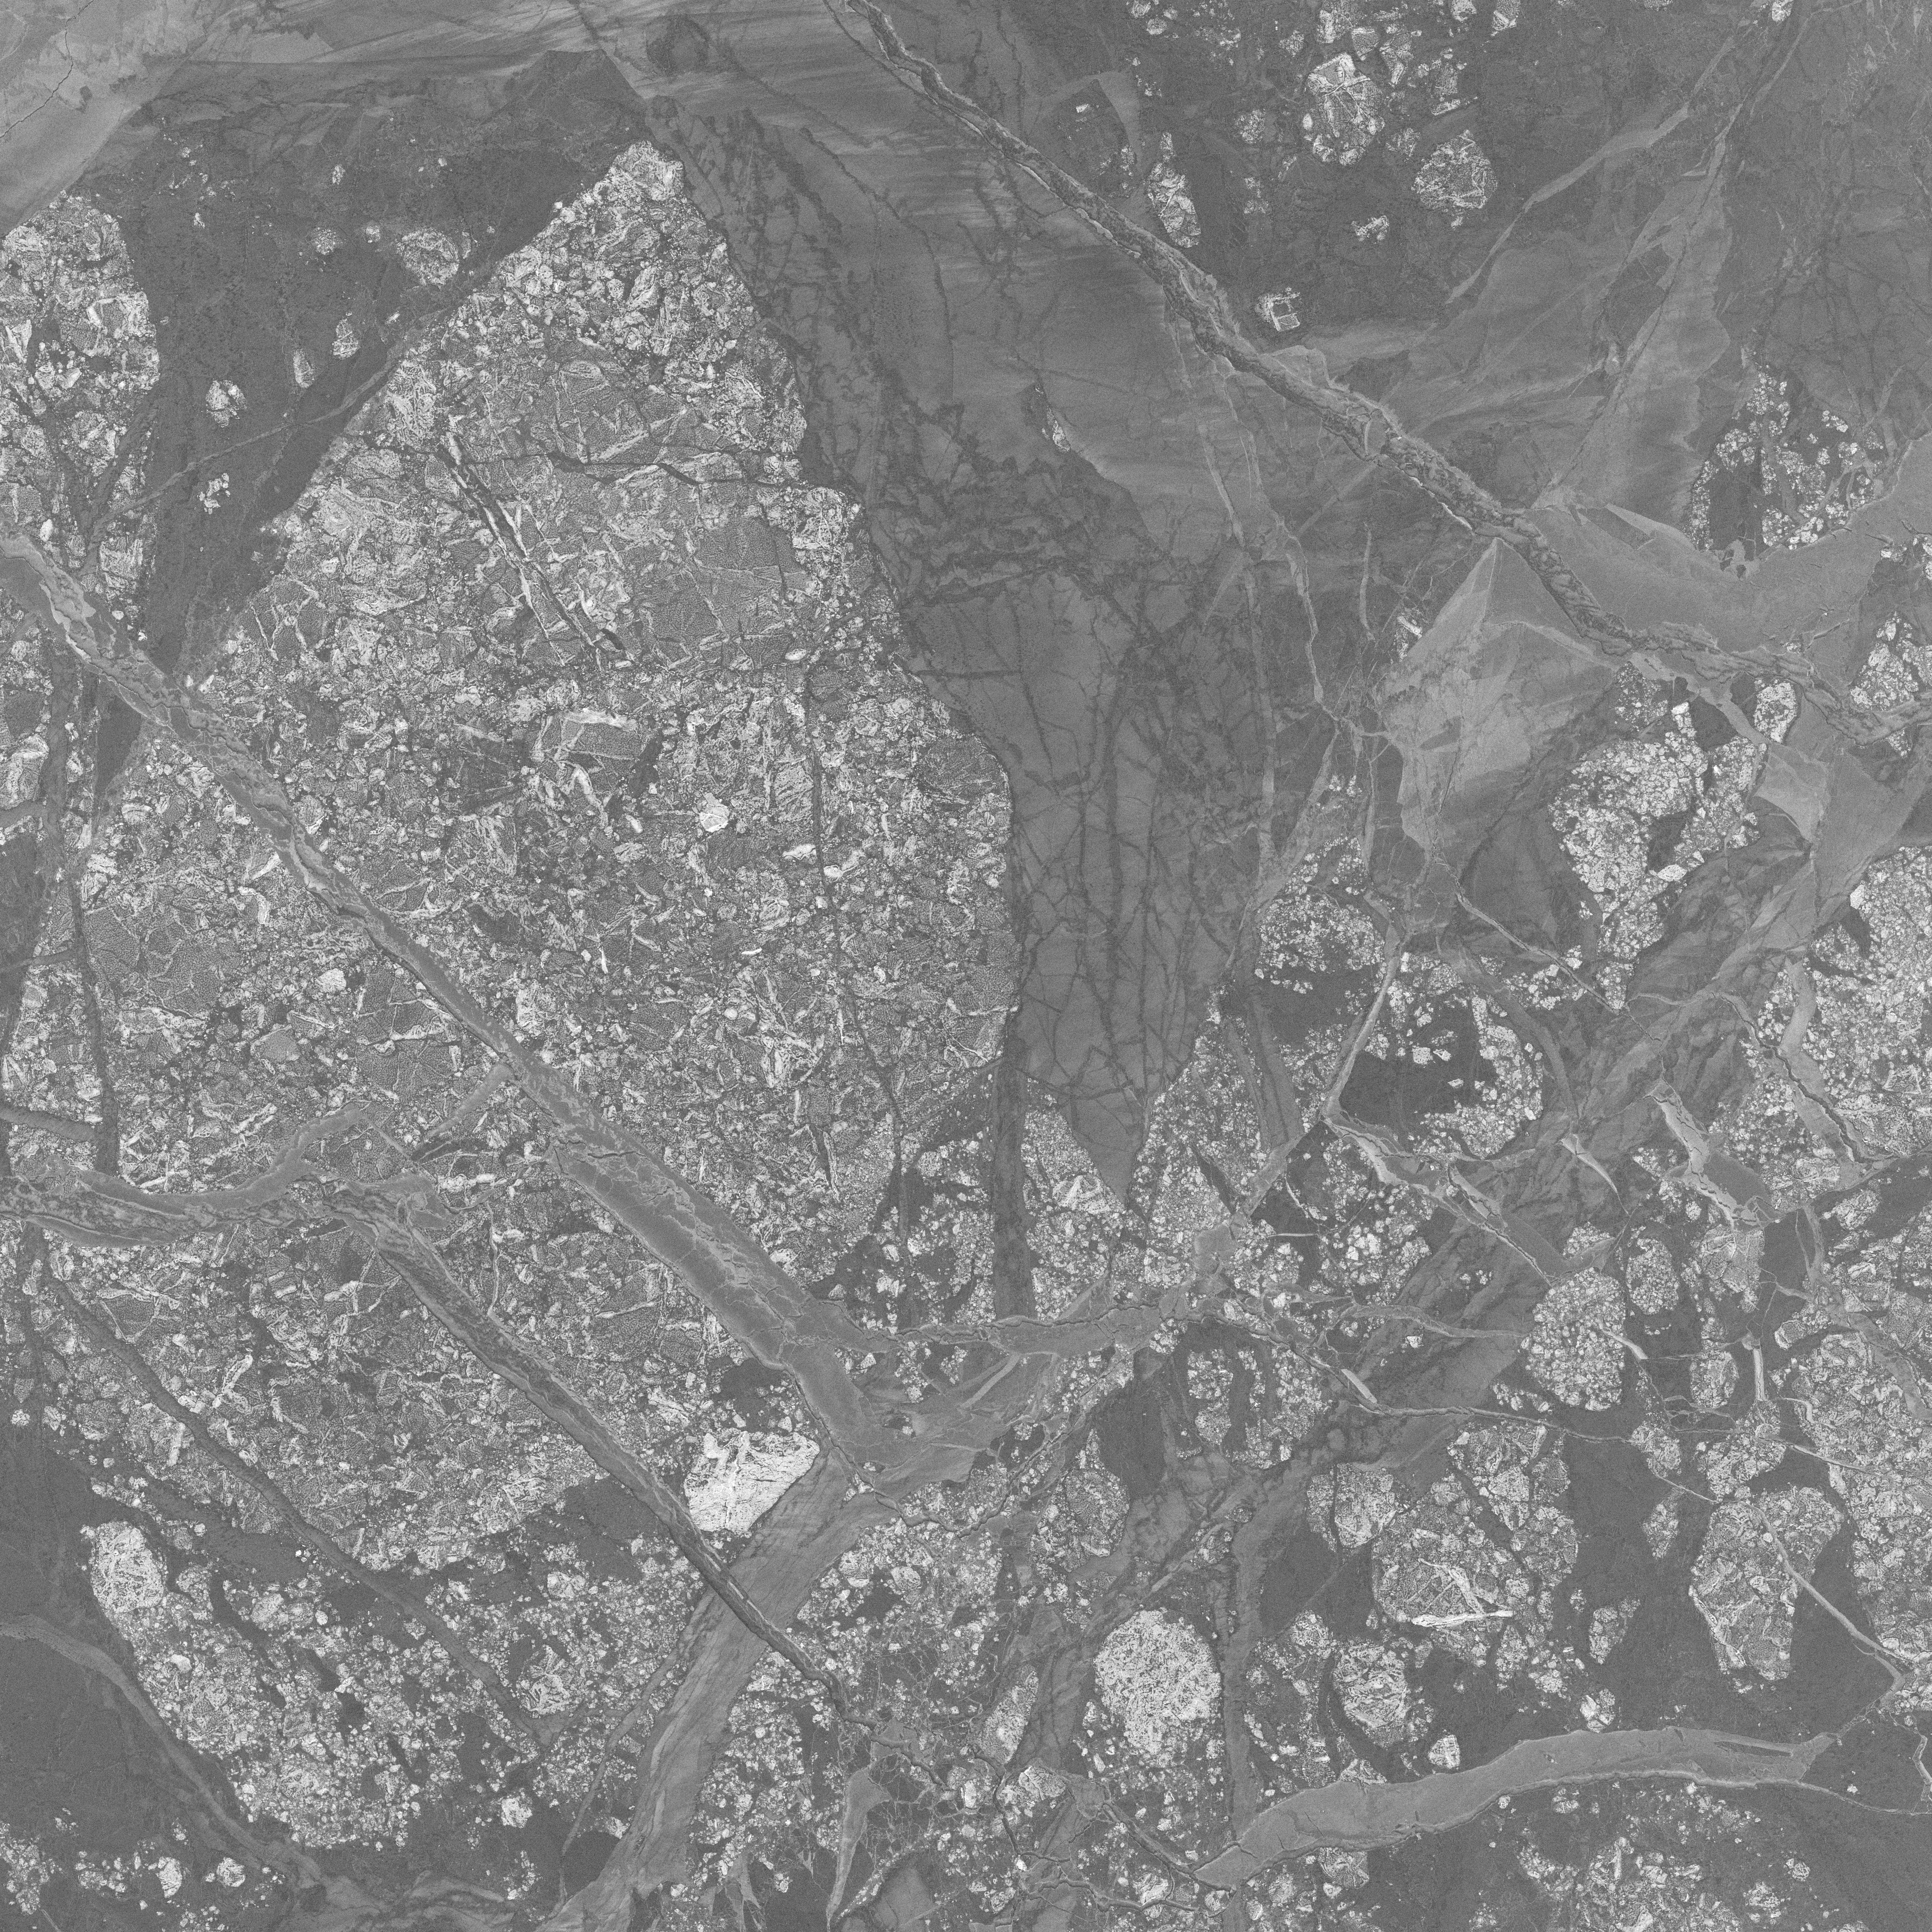
\includegraphics[width=.48\linewidth]{./research-resources/SAR/ICEYE_X13_QUICKLOOK_SLEA_3279210_20240119T023534.png}}
    \caption{(a), (b), (c), (d)}
    \label{gathered-sar}%
\end{figure}

\section {Laser Altimetry (IceSat-2)}



\begin{figure}[]
	\centering
	\includegraphics[width=.8\textwidth]{../research-resources/ice-sat-2/Surface Profiles.png}
	\caption{Ice Thicknesses}
	\label{fig:ice-thickness-gathered}
\end{figure}

------Default Text ----------

Provide in brief the background information for your work/field keeping in mind that maybe your readers do not have experience with topics your reference or address in your thesis. 

In the second part, provide a review of the state of the art relevant to your thesis. Here you present relevant research that relates to your work. 
